% Background. Standard formalisms only; the paper's own definitions (rule lists, certification,
% families with a vocabulary) go in the Problem section (sec:problem).

\section{Background}
\label{sec:background}

In this section, we introduce Markov decision processes and the grid world we use as a running example (\autoref{sec:bg-mdp}), and then probabilistic model checking (\autoref{sec:bg-pmc}).

\subsection{Markov Decision Processes}
\label{sec:bg-mdp}

A \textit{Markov decision process} (MDP) is a tuple $M = (S, s_0, A, P)$, where $S$ is a finite set of states, $s_0 \in S$ is the initial state, $A$ is a finite set of actions, and $P : S \times A \times S \to [0,1]$ gives the probability $P(s, a, s')$ of moving from $s$ to $s'$ when action $a$ is taken.
A \textit{strategy} $\sigma$ resolves the choice of action in each state, possibly depending on the history of the run and possibly at random.
Fixing a strategy turns $M$ into a Markov chain, which assigns a probability to every set of runs~\cite{TODO-Baier2008-principles}.
A \textit{parametric} MDP describes a family of MDPs whose parameters, such as the size of a map or the length of a game, determine each \textit{instance}~\cite{TODO-Azeem2025-123Go}.
Unlike in families that only vary transition probabilities~\cite{TODO-Andriushchenko2024-PoliciesGrowOnTrees}, the parameters may change the state space itself, so a strategy computed for one instance does not apply to another.

\textbf{Running Example:}
We use the stochastic grid world of prior work~\cite{TODO-predecessor-LLMTrust2026} as our running example (\autoref{fig:grid}).
An agent starts in the top-left cell of an $n \times n$ grid and must visit the goals $g_1, g_2, g_3$ in order.
In each step, it moves up, right, down or left.
A move succeeds with probability 0.7 and slips to either side with probability 0.15 each, and a move into the border or a static obstacle leaves the agent in place.
A moving obstacle patrols a fixed cycle of cells, advancing one cell per step, and the agent collides with it when both occupy the same cell.
A state records the agent's cell, which goals it has reached, and the position of the moving obstacle in its cycle.
The grid's size and layout are the parameters of the family, so larger grids have more states.

\begin{figure}[t]
\centering
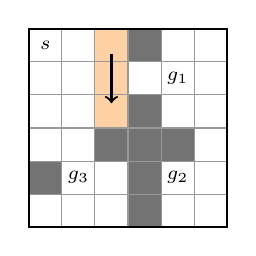
\begin{tikzpicture}[scale=0.42, every node/.style={font=\scriptsize}]
\foreach \c/\r in {3/0, 3/2, 2/3, 3/3, 4/3, 0/4, 3/4, 3/5}
  \fill[black!55] (\c, -\r) rectangle ++(1, -1);
\foreach \r in {0, 1, 2}
  \fill[orange!35] (2, -\r) rectangle ++(1, -1);
\draw[step=1, black!40] (0, 0) grid (6, -6);
\draw[thick] (0, 0) rectangle (6, -6);
\node at (0.5, -0.5) {$s$};
\node at (4.5, -1.5) {$g_1$};
\node at (4.5, -4.5) {$g_2$};
\node at (1.5, -4.5) {$g_3$};
\draw[->, thick] (2.5, -0.75) -- (2.5, -2.25);
\end{tikzpicture}
\caption{A 6$\times$6 instance of the grid world. The agent starts in cell $s$ and must visit $g_1$, $g_2$ and $g_3$ in order. Dark cells are static obstacles, and the moving obstacle patrols the shaded cells, down and back up.}
\label{fig:grid}
\end{figure}

\subsection{Probabilistic Model Checking}
\label{sec:bg-pmc}

Probabilistic model checkers such as PRISM~\cite{TODO-PRISM} compute the probability that the runs of an MDP satisfy a temporal property.
PRISM describes an MDP as a set of modules whose guarded commands update the state variables and carry action labels.
Commands with the same label in different modules synchronize, so a module can block an action in every state where its own guard for that action is false.
We express properties as path formulas $\psi$ of linear temporal logic (LTL)~\cite{TODO-Pnueli1977-LTL} over atomic propositions that label states, using the operators \textit{eventually} ($\mathbf{F}$), \textit{always} ($\mathbf{G}$) and \textit{until} ($\mathbf{U}$).
A \textit{requirement} $\varphi = P_{\bowtie \theta}[\psi]$, with $\bowtie\, \in \{\geq, \leq\}$, demands that the probability of $\psi$ meets the threshold $\theta$.
A strategy $\sigma$ satisfies $\varphi$ if $\mathit{Pr}^{\sigma}(\psi) \bowtie \theta$.
Since an MDP leaves the choice of actions open, PRISM computes the \textit{best case} and the \textit{worst case} of a requirement over all strategies, i.e., $\max_\sigma \mathit{Pr}^{\sigma}(\psi)$ and $\min_\sigma \mathit{Pr}^{\sigma}(\psi)$ for a lower bound, and the reverse for an upper bound.
If the worst case meets the threshold, every strategy satisfies the requirement~\cite{TODO-Baier2008-principles}.
PRISM can also return a strategy that attains the best case.
Bounds on expected rewards are handled in the same way, and we omit them for brevity.

A \textit{permissive strategy} allows a set of actions in each state rather than a single one~\cite{TODO-Draeger2015-permissive}.
Restricting an MDP to the actions a permissive strategy allows yields another MDP, whose strategies are exactly the strategies that only take allowed actions, with or without memory and randomization.
If the worst case of a requirement on the restricted MDP meets its threshold, every such strategy therefore satisfies the requirement.

In the running example, three kinds of requirements apply to each goal $g_k$.
With $\mathit{at}_k$ labeling the cell of $g_k$, the agent must eventually reach $g_k$, i.e., $P_{\geq 0.8}[\mathbf{F}\, \mathit{at}_k]$, and it must not enter $g_k$ before the earlier goals, e.g., $P_{\geq 0.8}[\neg \mathit{at}_2\ \mathbf{U}\ \mathit{at}_1]$ for the first two goals.
While heading to $g_k$, it must also avoid the moving obstacle, i.e., $P_{\geq 0.7}[\mathbf{G}\,(\mathit{seg}_k \Rightarrow \neg \mathit{collision})]$, where $\mathit{seg}_k$ holds in the states between reaching $g_{k-1}$ and reaching $g_k$.
Requiring collision avoidance per segment, rather than over the whole run, tells apart which part of a run is unsafe\todo{confirm this rationale; the predecessor paper's wording was ``per-segment obstacle avoidance''}.

PRISM computes these probabilities iteratively.
Standard value iteration stops when an iteration changes the values little, which does not bound the error, and on models where probability leaks away slowly it can stop far from the true value~\cite{TODO-Haddad2018-interval-iteration}.
Interval iteration instead approaches the value from both sides and stops once the two bounds are within a given precision, so the values it reports have a guaranteed error bound~\cite{TODO-Haddad2018-interval-iteration,TODO-Baier2017-interval-iteration}.
